% Options for packages loaded elsewhere
\PassOptionsToPackage{unicode}{hyperref}
\PassOptionsToPackage{hyphens}{url}
%
\documentclass[
  12pt,
]{article}
\usepackage{lmodern}
\usepackage{amssymb,amsmath}
\usepackage{ifxetex,ifluatex}
\ifnum 0\ifxetex 1\fi\ifluatex 1\fi=0 % if pdftex
  \usepackage[T1]{fontenc}
  \usepackage[utf8]{inputenc}
  \usepackage{textcomp} % provide euro and other symbols
\else % if luatex or xetex
  \usepackage{unicode-math}
  \defaultfontfeatures{Scale=MatchLowercase}
  \defaultfontfeatures[\rmfamily]{Ligatures=TeX,Scale=1}
\fi
% Use upquote if available, for straight quotes in verbatim environments
\IfFileExists{upquote.sty}{\usepackage{upquote}}{}
\IfFileExists{microtype.sty}{% use microtype if available
  \usepackage[]{microtype}
  \UseMicrotypeSet[protrusion]{basicmath} % disable protrusion for tt fonts
}{}
\makeatletter
\@ifundefined{KOMAClassName}{% if non-KOMA class
  \IfFileExists{parskip.sty}{%
    \usepackage{parskip}
  }{% else
    \setlength{\parindent}{0pt}
    \setlength{\parskip}{6pt plus 2pt minus 1pt}}
}{% if KOMA class
  \KOMAoptions{parskip=half}}
\makeatother
\usepackage{xcolor}
\IfFileExists{xurl.sty}{\usepackage{xurl}}{} % add URL line breaks if available
\IfFileExists{bookmark.sty}{\usepackage{bookmark}}{\usepackage{hyperref}}
\hypersetup{
  pdftitle={Exercise 1 Solutions},
  pdfauthor={Ian McCarthy, Econ 771},
  hidelinks,
  pdfcreator={LaTeX via pandoc}}
\urlstyle{same} % disable monospaced font for URLs
\usepackage[left=2cm,right=2cm,top=1cm,bottom=2cm]{geometry}
\usepackage{color}
\usepackage{fancyvrb}
\newcommand{\VerbBar}{|}
\newcommand{\VERB}{\Verb[commandchars=\\\{\}]}
\DefineVerbatimEnvironment{Highlighting}{Verbatim}{commandchars=\\\{\}}
% Add ',fontsize=\small' for more characters per line
\usepackage{framed}
\definecolor{shadecolor}{RGB}{248,248,248}
\newenvironment{Shaded}{\begin{snugshade}}{\end{snugshade}}
\newcommand{\AlertTok}[1]{\textcolor[rgb]{0.94,0.16,0.16}{#1}}
\newcommand{\AnnotationTok}[1]{\textcolor[rgb]{0.56,0.35,0.01}{\textbf{\textit{#1}}}}
\newcommand{\AttributeTok}[1]{\textcolor[rgb]{0.77,0.63,0.00}{#1}}
\newcommand{\BaseNTok}[1]{\textcolor[rgb]{0.00,0.00,0.81}{#1}}
\newcommand{\BuiltInTok}[1]{#1}
\newcommand{\CharTok}[1]{\textcolor[rgb]{0.31,0.60,0.02}{#1}}
\newcommand{\CommentTok}[1]{\textcolor[rgb]{0.56,0.35,0.01}{\textit{#1}}}
\newcommand{\CommentVarTok}[1]{\textcolor[rgb]{0.56,0.35,0.01}{\textbf{\textit{#1}}}}
\newcommand{\ConstantTok}[1]{\textcolor[rgb]{0.00,0.00,0.00}{#1}}
\newcommand{\ControlFlowTok}[1]{\textcolor[rgb]{0.13,0.29,0.53}{\textbf{#1}}}
\newcommand{\DataTypeTok}[1]{\textcolor[rgb]{0.13,0.29,0.53}{#1}}
\newcommand{\DecValTok}[1]{\textcolor[rgb]{0.00,0.00,0.81}{#1}}
\newcommand{\DocumentationTok}[1]{\textcolor[rgb]{0.56,0.35,0.01}{\textbf{\textit{#1}}}}
\newcommand{\ErrorTok}[1]{\textcolor[rgb]{0.64,0.00,0.00}{\textbf{#1}}}
\newcommand{\ExtensionTok}[1]{#1}
\newcommand{\FloatTok}[1]{\textcolor[rgb]{0.00,0.00,0.81}{#1}}
\newcommand{\FunctionTok}[1]{\textcolor[rgb]{0.00,0.00,0.00}{#1}}
\newcommand{\ImportTok}[1]{#1}
\newcommand{\InformationTok}[1]{\textcolor[rgb]{0.56,0.35,0.01}{\textbf{\textit{#1}}}}
\newcommand{\KeywordTok}[1]{\textcolor[rgb]{0.13,0.29,0.53}{\textbf{#1}}}
\newcommand{\NormalTok}[1]{#1}
\newcommand{\OperatorTok}[1]{\textcolor[rgb]{0.81,0.36,0.00}{\textbf{#1}}}
\newcommand{\OtherTok}[1]{\textcolor[rgb]{0.56,0.35,0.01}{#1}}
\newcommand{\PreprocessorTok}[1]{\textcolor[rgb]{0.56,0.35,0.01}{\textit{#1}}}
\newcommand{\RegionMarkerTok}[1]{#1}
\newcommand{\SpecialCharTok}[1]{\textcolor[rgb]{0.00,0.00,0.00}{#1}}
\newcommand{\SpecialStringTok}[1]{\textcolor[rgb]{0.31,0.60,0.02}{#1}}
\newcommand{\StringTok}[1]{\textcolor[rgb]{0.31,0.60,0.02}{#1}}
\newcommand{\VariableTok}[1]{\textcolor[rgb]{0.00,0.00,0.00}{#1}}
\newcommand{\VerbatimStringTok}[1]{\textcolor[rgb]{0.31,0.60,0.02}{#1}}
\newcommand{\WarningTok}[1]{\textcolor[rgb]{0.56,0.35,0.01}{\textbf{\textit{#1}}}}
\usepackage{longtable,booktabs}
% Correct order of tables after \paragraph or \subparagraph
\usepackage{etoolbox}
\makeatletter
\patchcmd\longtable{\par}{\if@noskipsec\mbox{}\fi\par}{}{}
\makeatother
% Allow footnotes in longtable head/foot
\IfFileExists{footnotehyper.sty}{\usepackage{footnotehyper}}{\usepackage{footnote}}
\makesavenoteenv{longtable}
\usepackage{graphicx}
\makeatletter
\def\maxwidth{\ifdim\Gin@nat@width>\linewidth\linewidth\else\Gin@nat@width\fi}
\def\maxheight{\ifdim\Gin@nat@height>\textheight\textheight\else\Gin@nat@height\fi}
\makeatother
% Scale images if necessary, so that they will not overflow the page
% margins by default, and it is still possible to overwrite the defaults
% using explicit options in \includegraphics[width, height, ...]{}
\setkeys{Gin}{width=\maxwidth,height=\maxheight,keepaspectratio}
% Set default figure placement to htbp
\makeatletter
\def\fps@figure{htbp}
\makeatother
\setlength{\emergencystretch}{3em} % prevent overfull lines
\providecommand{\tightlist}{%
  \setlength{\itemsep}{0pt}\setlength{\parskip}{0pt}}
\setcounter{secnumdepth}{-\maxdimen} % remove section numbering
\usepackage{setspace}
\usepackage{titlesec}
\titlespacing{\title}{0pt}{\parskip}{-\parskip}
\titlespacing{\section}{0pt}{12pt plus 2pt minus 1pt}{0pt plus 1pt minus 1pt}
\titlespacing{\subsection}{0pt}{12pt plus 2pt minus 1pt}{0pt plus 1pt minus 1pt}
\titlespacing{\subsubsection}{0pt}{12pt plus 2pt minus 1pt}{0pt plus 1pt minus 1pt}
\usepackage{float}
\usepackage{booktabs}
\usepackage{longtable}
\usepackage{array}
\usepackage{multirow}
\usepackage{wrapfig}
\usepackage{float}
\usepackage{colortbl}
\usepackage{pdflscape}
\usepackage{tabu}
\usepackage{threeparttable}
\usepackage{threeparttablex}
\usepackage[normalem]{ulem}
\usepackage{makecell}
\usepackage{xcolor}

\title{Exercise 1 Solutions}
\author{Ian McCarthy, Econ 771}
\date{Fall 2020}

\begin{document}
\maketitle

\setstretch{1.5}

\hypertarget{overview}{%
\section{Overview}\label{overview}}

This document lays out my approach to addressing the questions in Exercise 1. There are lots of ways to answer these problems and build the data, especially in \texttt{R}! My way of answering the questions is just one of many.

I also have a particular workflow that you may or may not choose to adopt. That workflow is to do all of my analysis seperately from my markdown document. I really don't like seeing huge markdown documents constantly going in and out of data work and discussion. It's also not feasible to work with really large data within the markdown document. So, I do all of the analysis, remove any large objects (including the data), keep only the relevant objects for the final markdown (figures, tables, specific numbers or statistics), and then save the workspace. Then I load the workspace into my markdown document.

\hypertarget{data}{%
\section{Data}\label{data}}

Before we get into the specific questions for this assignment, let's briefly go through the data. My code files for the IPPS and POS data are included in the classroom repo under the filenames \emph{1\_ipps.R} and \emph{2\_pos.R}.

\hypertarget{ipps-data}{%
\subsubsection{IPPS Data}\label{ipps-data}}

The IPPS data are pretty straightforward except for some slight changes in variable names over time. For example, ``Provider Type'' is missing in years 1986 through 1983; it is named ``provtype'' in years 1994 through 2000; and it is renamed ``ptype'' from 2001 onward.

\hypertarget{pos-data}{%
\subsubsection{POS Data}\label{pos-data}}

The POS data may be a little troublesome to download because there are lots of different versions of the same datasets. From the \href{https://data.nber.org/data/provider-of-services.html}{NBER POS website}, I extracted the ``csvYYYY'' files from 1984 through 1990. Starting in 1991, there are two links for the csv files -- a ``csv'' and a ``PROV''. The ``PROV'' link is active but the datasets are empty in some of the earlier years, so I used the ``csv'' links in all cases. These links are to a crosswalk version of the data, in which the NBER tried to assign a consistent name to each variable in the POS data. The original, raw POS files had variable names like, ``prov0028'', but they changed to mnemonic style names in 2011. The crosswalk files are intended to make it easier to merge historic data with data from 2011 onward. These versions of the data are what I have made available in the AWS AMI.

The POS data are supposed to be updated regularly, meaning that you should only need the most recent version of the data; however, that doesn't appear to be the case as some provider numbers only show up in the earlier years. It appears that once a hospital has been closed for a sufficiently long time, it no longer appears in the POS. Still, since the values are intended to be replaced every year for a given POS, there are \textbf{a lot} of duplicates. In my code file, I read in all of the data, recode the relevant variables, and then drop the duplicates.

\hypertarget{final-dataset}{%
\subsubsection{Final dataset}\label{final-dataset}}

Once you have the ipps and POS data ready, you just have to merge the two. The easiest way to do this in our case is to merge on provider number and year. Here's my code to merge the three datasets:

\setstretch{1}

\begin{Shaded}
\begin{Highlighting}[]
\NormalTok{full.data \textless{}{-}}\StringTok{ }\NormalTok{final.pos.data }\OperatorTok{\%\textgreater{}\%}
\StringTok{  }\KeywordTok{left\_join}\NormalTok{(final.ipps.data, }\DataTypeTok{by=}\KeywordTok{c}\NormalTok{(}\StringTok{"provider"}\NormalTok{, }\StringTok{"year"}\NormalTok{))}
\end{Highlighting}
\end{Shaded}

\setstretch{1.5}

\hypertarget{question-and-answers}{%
\section{Question and Answers}\label{question-and-answers}}

\hypertarget{question-1.}{%
\subsubsection{Question 1.}\label{question-1.}}

\textbf{Provide and discuss a table of simple summary statistics showing the mean, standard deviation, min, and max of the case mix index and disproportionate share across years. Show these statistics overall and separately by hospital ownership type.}

Table \ref{tab:sum-stats} presents the mean, standard deviation, min, and max of the relevant variables. Note that disproportionate share information isn't available in the data until 1994, so the summary stats are missing until that year. We see from the table that the mean case mix index is increasing over time, which means that people are getting sicker. We also see that the mean DSH has increased over time, from about 23\% to 30\% in 2018.

\hypertarget{question-2.}{%
\subsubsection{Question 2.}\label{question-2.}}

\textbf{Create a figure showing the average hospital disproportionate shares from 1986 to 2018. Show this trend separately by hospital ownership type (private not for profit and private for profit).}

A table is not the best way to present summary statistics over several years like this. So, let's do that in a figure instead. Figures \ref{fig:cmi-plot} and \ref{fig:dsh-plot} present the average Case Mix Index and disproportionate shares, respectively, for each year. Each figure presents two lines, one showing the mean among for profit hosptials and the other showing the mean for private not-for-profit hospitals (labeled simply as ``Non Profit'' in the figures).

\hypertarget{question-3}{%
\subsubsection{Question 3}\label{question-3}}

\textbf{Using a simple DD identification strategy, estimate the effect of Medicaid expansion on the hospital disproportionate share percentage. Do these effects differ by profit status (i.e., re-estimate with a DDD using profit status)? Focus your analysis on the years from 2005 through 2018.}

The disproportionate share program is actually two programs - a Medicaid and a Medicare program. The Medicare DSH program, which is what is relevant for the IPPS data, calculates a hospital's disproportionate share percentage based on the share of Medicare patients that are eligible for SSI as well as the number of Medicaid patients. Since not all states expanded Medicaid in 2014, we can use the ACA Medicaid expansion as a treatment and estimate the effect of Medicaid expansion on hospital DSH percentage (which should be positive, since more people would be on Medicaid).

Before thinking of any type of regression, it's always a good idea just to summarize the key parts of your data. In this case, we want to know how DSH changed from before and after 2014, separately by states that expanded and didn't expand Medicaid.

Table \ref{tab:dd-table} presents the 2x2 DD chart with pre/post, treatment/control averages. From these averages, our DD estimate for the effect of Medicaid expansion on DSH would be 0.00687.

We can estimate this effect in a regression setting based on the specification in Equation \eqref{eq:dd1}:
\begin{equation}
DSH_{ht} = \alpha Expand_{s} + \beta 1(t\geq 2014) + \delta Expand_{s} \times 1(t\geq 2014) + \varepsilon_{ht}, \label{eq:dd1}
\end{equation}
where \(DSH_{ht}\) is the Disproportionate Share percent for hospital \(h\) at time \(t\), \(Expand_{s}\) denotes an indicator set to 1 if the hospital is part of a Medicaid expansion state and 0 otherwise, and \(1(t\geq 2014)\) denotes an indicator for the treatment period (after the Medicaid expansion in 2014).

Since we have multiple years of data, a more general specification is presented in equation \eqref{eq:dd2}:
\begin{equation}
DSH_{ht} = \delta Expand_{s} \times (t>2014) + \lambda_{h} + \gamma_{t} + \varepsilon_{ij}, \label{eq:dd2}
\end{equation}
where \(\lambda_{h}\) and \(\gamma_{t}\) denote hospital and year fixed effects, respectively. Hopefully it is clear that Equation \eqref{eq:dd2} subsumes Equation \eqref{eq:dd1} as a special case.

The estimates for \(\delta\) from each specification are presented in Table \ref{tab:dd-regs}. These estimates confirm our original estimates in the 2x2 DD table, where we find a relatively large increase in DSH among hospitals in expansion states.

We can also separate this effect by for profit status, in which we use ownership type to create a 3rd category of interest (hence, the triple difference, or difference-in-difference-in-difference, or just DDD). Ownership type shouldn't change much over time, but it can. This isn't good for a DDD, because you'd like all of your groups to be stable. I'm going to deal with this issue in a haphazard way and just re-define ``for profit'' as a hospital that is ever for profit in the treatment period (2014 and after). The final specification we're estimating is written in Equation \eqref{eq:ddd}.
\begin{align}
DSH_{ht} = &\beta_{1} Expand_{s} + \beta_{2} 1(t\geq 2014) + \beta_{3} Expand_{s} \times 1(t\geq 2014) + \nonumber \\
& \beta_{4} ForProfit_{h} + \beta_{5} ForProfit_{h} \times 1(t\geq 2014) + \nonumber \\
& \delta ForProfit_{h} \times Expand_{s} \times 1(t\geq 2014) +  \varepsilon_{ht}, \label{eq:ddd}
\end{align}
Results from estimating this equation are provided Table \ref{tab:ddd-regs}, where we see that for profit hospitals indeed have a larger estimated response than not-for-profit hospitals. In fact, based on this simple DDD specification, the effect is almost entirely driven by for profit hospitals.

\hypertarget{question-4}{%
\subsubsection{Question 4}\label{question-4}}

\textbf{Estimate an ``event study'' version of the DD model from part 3. Focus only on states that expanded in 2014 that those that have never expanded.}

Event study estimates for 2014 expansion are presented in Figure \ref{fig:event-study1}.

\hypertarget{question-5}{%
\subsubsection{Question 5}\label{question-5}}

\textbf{Estimate another event study where you allow for differential treatment timing and incorporate all states.}

Event study estimates for all expansion states (time varying treatment) are presented in Figure \ref{fig:event-study2}. Here, time of 0 denotes the start of treatment, so \emph{t-1} is the baseline period for which every other period is estimated. That's why the coefficient for the \emph{t-1} period is normalized to 0. Note that the full data run from 2005 to 2018, so DSH in period \emph{t-12} is only observed for states that expanded in 2016. Since very few states expanded in 2017 or 2018, I've lumped all of those states into the \emph{t-12} period.

\newpage
\setstretch{1}

\hypertarget{tables-and-figures}{%
\section{Tables and Figures}\label{tables-and-figures}}

\begin{table}[H]

\caption{\label{tab:sum-stats}Summary Statistics}
\centering
\begin{tabular}[t]{lrrrrrrrr}
\toprule
\multicolumn{1}{c}{ } & \multicolumn{4}{c}{Case Mix Index} & \multicolumn{4}{c}{Disproportionate Share} \\
\cmidrule(l{3pt}r{3pt}){2-5} \cmidrule(l{3pt}r{3pt}){6-9}
Year & Mean & Std. Dev. & Min & Max & Mean & Std. Dev. & Min & Max\\
\midrule
1986 & 1.12 & 0.14 & 0.59 & 2.23 &  &  &  & \\
1987 & 1.15 & 0.15 & 0.72 & 2.15 &  &  &  & \\
1988 & 1.18 & 0.17 & 0.61 & 2.16 &  &  &  & \\
1989 & 1.20 & 0.18 & 0.63 & 2.28 &  &  &  & \\
1990 & 1.20 & 0.19 & 0.56 & 3.21 &  &  &  & \\
\addlinespace
1991 & 1.22 & 0.21 & 0.50 & 2.75 &  &  &  & \\
1992 & 1.23 & 0.22 & 0.48 & 2.61 &  &  &  & \\
1993 & 1.20 & 0.24 & 0.47 & 4.42 &  &  &  & \\
1994 & 1.22 & 0.24 & 0.44 & 3.72 & 0.23 & 0.18 & 0 & 1.60\\
1995 & 1.22 & 0.25 & 0.41 & 2.87 & 0.24 & 0.19 & 0 & 1.66\\
\addlinespace
1996 & 1.24 & 0.25 & 0.31 & 3.10 & 0.24 & 0.19 & 0 & 1.64\\
1997 & 1.25 & 0.26 & 0.41 & 3.67 & 0.25 & 0.19 & 0 & 1.28\\
1998 & 1.27 & 0.40 & 0.40 & 15.93 & 0.24 & 0.19 & 0 & 1.33\\
1999 & 1.27 & 0.35 & 0.42 & 16.34 & 0.24 & 0.18 & 0 & 1.30\\
2000 & 1.26 & 0.28 & 0.42 & 3.71 & 0.24 & 0.18 & 0 & 1.28\\
\addlinespace
2001 & 1.25 & 0.28 & 0.42 & 3.83 & 0.24 & 0.18 & 0 & 1.52\\
2002 & 1.25 & 0.29 & 0.29 & 3.80 & 0.23 & 0.18 & 0 & 1.29\\
2003 & 1.26 & 0.27 & 0.39 & 2.99 & 0.24 & 0.18 & 0 & 1.34\\
2004 & 1.28 & 0.28 & 0.40 & 4.02 & 0.25 & 0.18 & 0 & 1.32\\
2005 & 1.30 & 0.29 & 0.36 & 3.53 & 0.26 & 0.18 & 0 & 1.24\\
\addlinespace
2006 & 1.33 & 0.30 & 0.36 & 3.07 & 0.26 & 0.18 & 0 & 1.23\\
2007 & 1.36 & 0.31 & 0.41 & 7.52 & 0.27 & 0.18 & 0 & 1.24\\
2008 & 1.36 & 0.31 & 0.45 & 4.13 & 0.27 & 0.18 & 0 & 1.20\\
2009 & 1.36 & 0.31 & 0.58 & 3.74 & 0.27 & 0.18 & 0 & 1.22\\
2010 & 1.41 & 0.34 & 0.50 & 3.74 & 0.27 & 0.18 & 0 & 1.22\\
\addlinespace
2011 & 1.43 & 0.33 & 0.57 & 3.75 & 0.28 & 0.18 & 0 & 1.24\\
2012 & 1.45 & 0.33 & 0.60 & 4.28 & 0.28 & 0.18 & 0 & 1.24\\
2013 & 1.46 & 0.33 & 0.59 & 3.76 & 0.28 & 0.18 & 0 & 1.19\\
2014 & 1.48 & 0.35 & 0.56 & 3.80 & 0.28 & 0.18 & 0 & 1.23\\
2015 & 1.51 & 0.35 & 0.65 & 3.97 & 0.28 & 0.18 & 0 & 1.22\\
\addlinespace
2016 & 1.53 & 0.36 & 0.59 & 4.36 & 0.29 & 0.18 & 0 & 1.49\\
2017 & 1.54 & 0.37 & 0.61 & 3.97 & 0.30 & 0.18 & 0 & 1.23\\
2018 & 1.58 & 0.37 & 0.65 & 4.88 & 0.30 & 0.18 & 0 & 1.19\\
\bottomrule
\end{tabular}
\end{table}

\newpage

\begin{table}[H]

\caption{\label{tab:dd-table}DD Table for Medicaid Expansion}
\centering
\begin{tabular}[t]{lll}
\toprule
Group & Pre & Post\\
\midrule
Non-expansion & 0.28 & 0.27\\
Expansion & 0.29 & 0.29\\
\bottomrule
\end{tabular}
\end{table}

\newpage

\begin{table}[H] \centering 
  \caption{Difference-in-Differences Estimates} 
  \label{tab:dd-regs} 
\begin{tabular}{@{\extracolsep{5pt}}lcc} 
\\[-1.8ex]\hline 
\hline \\[-1.8ex] 
\\[-1.8ex] & \multicolumn{2}{c}{Disproportionate Share} \\ 
\\[-1.8ex] & (1) & (2)\\ 
\hline \\[-1.8ex] 
 After 2014 & 0.001 &  \\ 
  & (0.003) &  \\ 
  Expansion & 0.014$^{***}$ &  \\ 
  & (0.002) &  \\ 
  Treatment Effect & 0.040$^{***}$ & 0.035$^{***}$ \\ 
  & (0.004) & (0.001) \\ 
  Constant & 0.268$^{***}$ &  \\ 
  & (0.002) &  \\ 
 \hline \\[-1.8ex] 
Model & DD & DD, FE \\ 
Observations & 42,698 & 42,698 \\ 
\hline 
\hline \\[-1.8ex] 
\textit{Note:}  & \multicolumn{2}{r}{$^{*}$p$<$0.1; $^{**}$p$<$0.05; $^{***}$p$<$0.01} \\ 
\end{tabular} 
\end{table}

\newpage

\begin{table}[H] \centering 
  \caption{Triple Differences Estimates} 
  \label{tab:ddd-regs} 
\begin{tabular}{@{\extracolsep{5pt}}lc} 
\\[-1.8ex]\hline 
\hline \\[-1.8ex] 
\\[-1.8ex] & Disproportionate Share \\ 
\hline \\[-1.8ex] 
 After 2014 & 0.025$^{***}$ \\ 
  & (0.005) \\ 
  Expansion & 0.025$^{***}$ \\ 
  & (0.003) \\ 
  Treatment & 0.007 \\ 
  & (0.005) \\ 
  Ever FP & 0.046$^{***}$ \\ 
  & (0.003) \\ 
  After 2014 x FP & $-$0.049$^{***}$ \\ 
  & (0.006) \\ 
  Treat x FP & 0.065$^{***}$ \\ 
  & (0.008) \\ 
  Constant & 0.236$^{***}$ \\ 
  & (0.002) \\ 
 \hline \\[-1.8ex] 
Observations & 27,821 \\ 
\hline 
\hline \\[-1.8ex] 
\textit{Note:}  & \multicolumn{1}{r}{$^{*}$p$<$0.1; $^{**}$p$<$0.05; $^{***}$p$<$0.01} \\ 
\end{tabular} 
\end{table}

\newpage

\begin{figure}
\centering
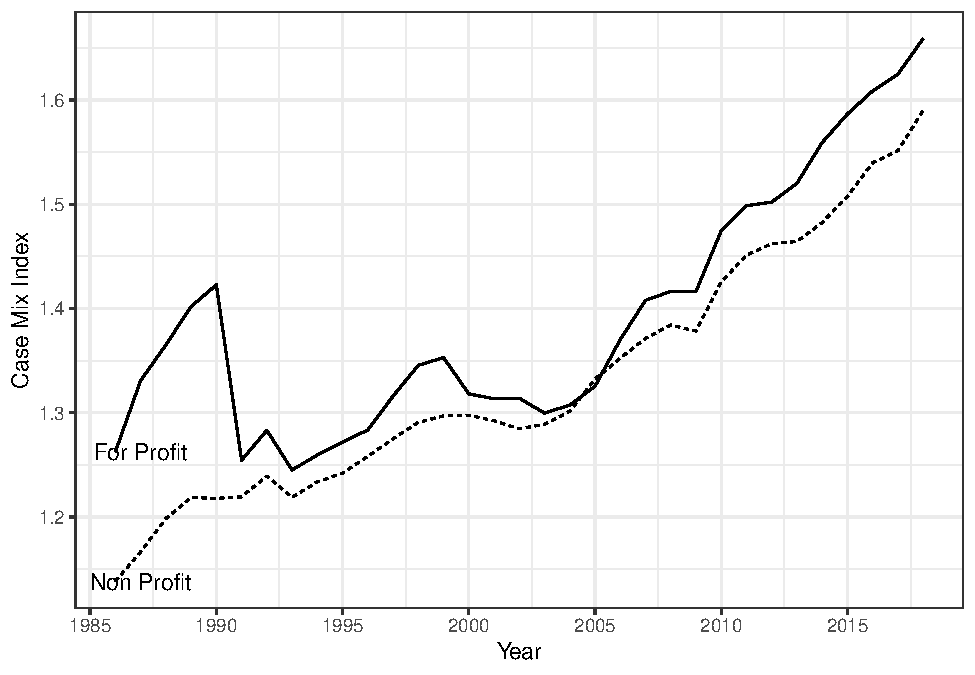
\includegraphics{solutions_files/figure-latex/cmi-plot-1.pdf}
\caption{\label{fig:cmi-plot}Mean Case Mix Index by Year and Profit Status}
\end{figure}

\newpage

\begin{figure}
\centering
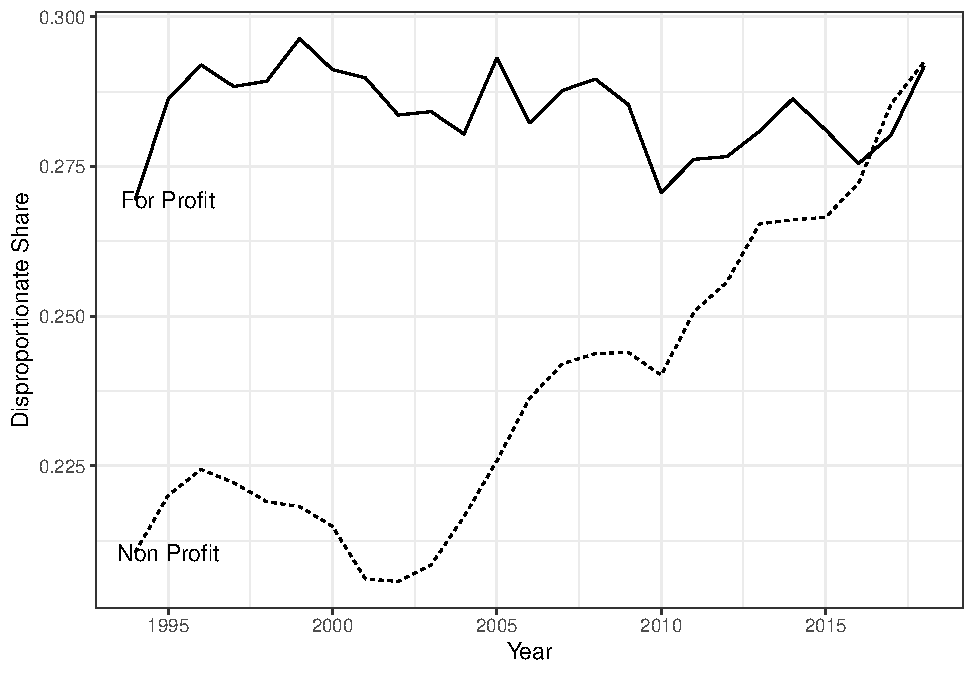
\includegraphics{solutions_files/figure-latex/dsh-plot-1.pdf}
\caption{\label{fig:dsh-plot}Mean Disproportionate Share by Year and Profit Status}
\end{figure}

\newpage

\begin{figure}
\centering
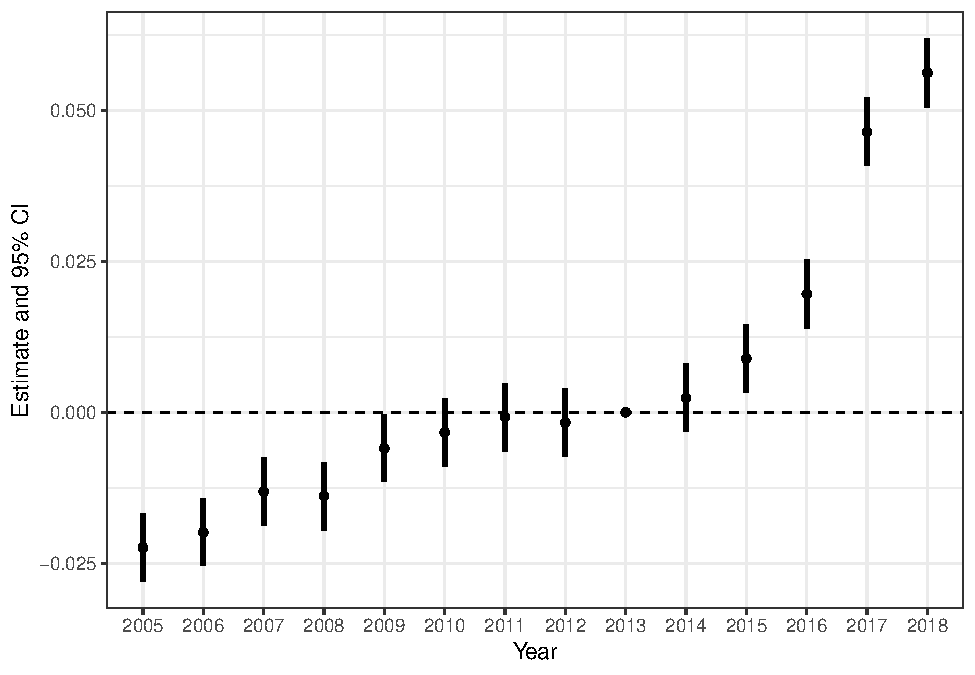
\includegraphics{solutions_files/figure-latex/event-study1-1.pdf}
\caption{\label{fig:event-study1}Event Study for 2014 Treatment Group}
\end{figure}

\newpage

\begin{figure}
\centering
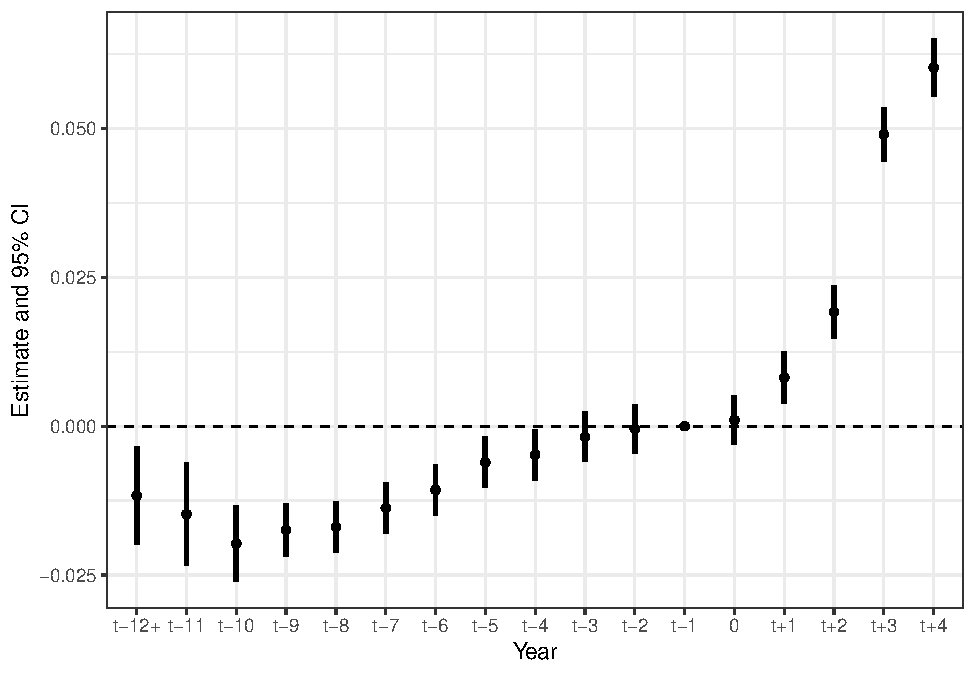
\includegraphics{solutions_files/figure-latex/event-study2-1.pdf}
\caption{\label{fig:event-study2}Event Study for All Expansion States}
\end{figure}

\end{document}
